\section{Methodology}
This section describes the methods and procedures used for generating product reviews on e-commerce platforms through the use of Large Language Models (LLMs). It covers all stages of the process, from data collection and preparation to the evaluation of the fine-tuned models.
\\\\
Since the dataset has been generated from scratch, the procedure for data acquisition and generation is detailed, as well as the cleaning and structuring of the data. The techniques used for model tuning are then described, including the selection of hyperparameters and optimization methods. Finally, the evaluation metrics used to analyze the outcomes are presented.
\\\\
Figure \ref{fig:MethodologyFlowchart} displays a flowchart that summarizes the methodology followed in this study. The explanation begins with data extraction, followed by data preparation, model tuning, and finally, the evaluation of the results obtained.
\\\\
This comprehensive approach ensures a systematic and thorough exploration of the potential and limitations of LLMs in generating meaningful and reliable product reviews, highlighting both the technological advancements and the practical challenges encountered during implementation.

\begin{figure}[H]
    \centering
    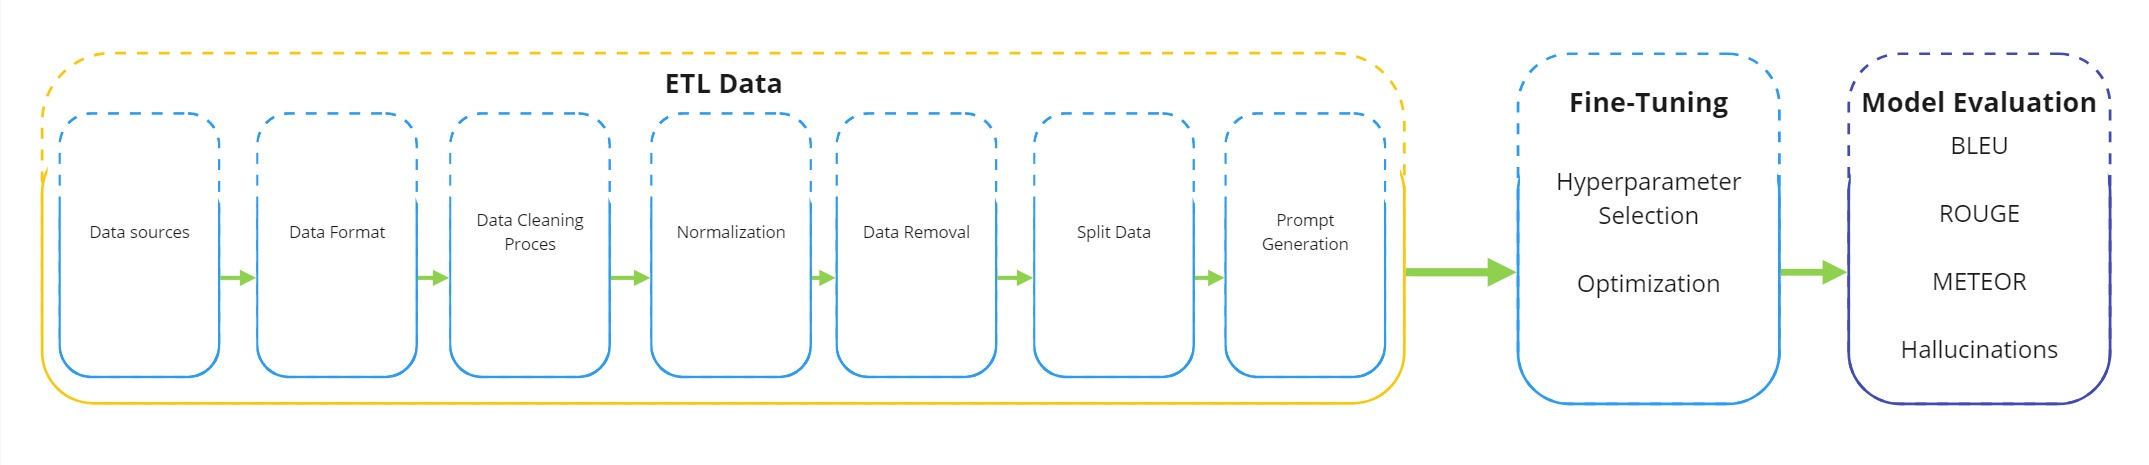
\includegraphics[width=12cm]{images/Methodology.jpg}
    \caption{Methodology Flowchart}
    \label{fig:MethodologyFlowchart}
\end{figure}
